\section{phpLogCon}
\subsection{Überblick}
\begin{frame}
	\frametitle{phpLogCon}
	\framesubtitle{"Uberblick}
	\begin{itemize}
		\item php-Webinterface mit MySql-Datenbank
		\item tabellarische Darstellung
		\item personalsierbare Ansichten und Filterungen
		\item Diagrammauswertung für besseren Überblick
	\end{itemize}
\end{frame}

\subsection{Installation}
\begin{frame}[fragile]
	\frametitle{phpLogCon}
	\framesubtitle{Installation}
	Die Installation ist so nur unter Ubuntu möglich
	\begin{block}{Debian, Ubuntu}
	\begin{verbatim}
		Lamp Server
		apt-get install rsyslog-mysql
		apt-get install rsyslog-relp
	\end{verbatim}
	\end{block}
\end{frame}

\subsection{Webinterface}
\begin{frame}
	\frametitle{phpLogCon}
	\framesubtitle{Webinterface}
	\begin{itemize}
		\item Suche
		\item Meldungen
		\item Statistiken
		\item Administration
	\end{itemize}
\end{frame}

\subsubsection{Suche}
\begin{frame}
	\frametitle{phpLogCon - Webinterface}
	\framesubtitle{Suche}
	\begin{center}
		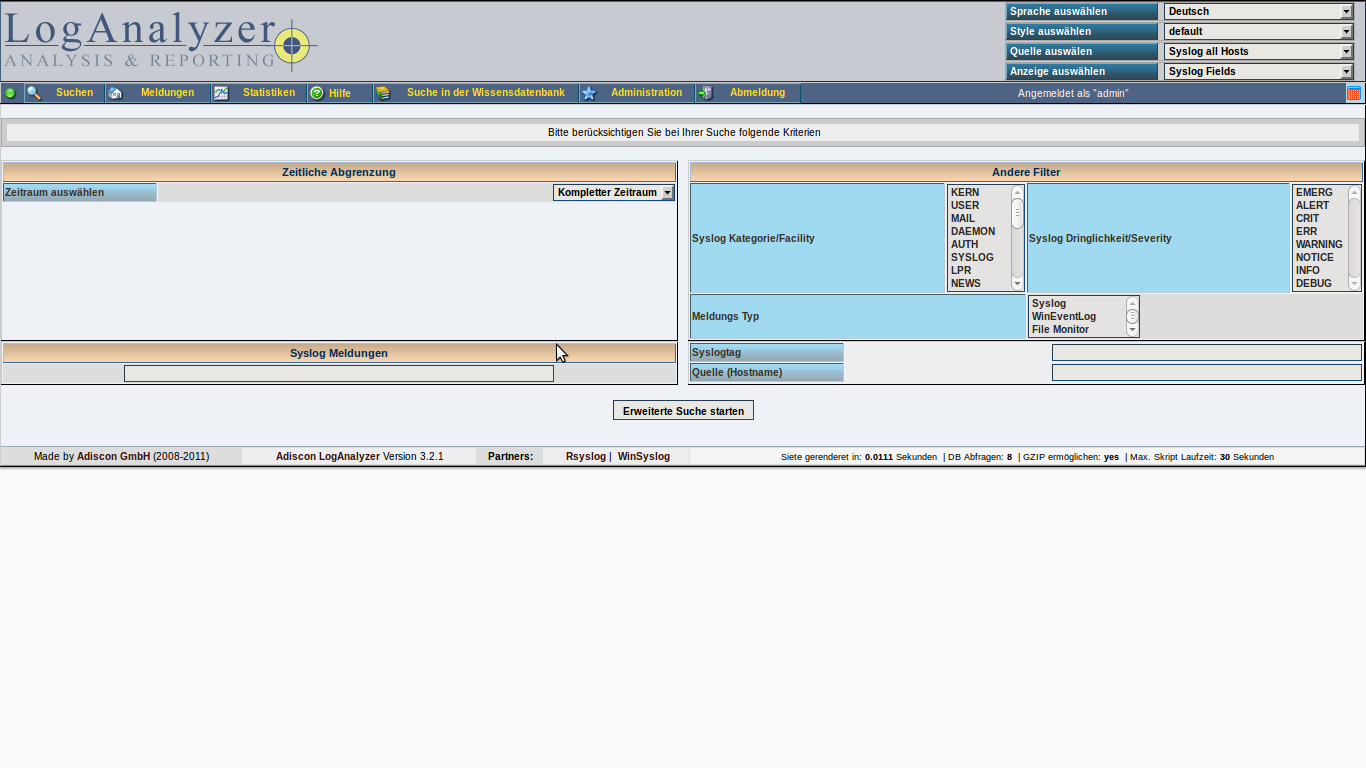
\includegraphics[width=\linewidth]{images/phplogcon_suche.eps}
	\end{center}
\end{frame}

\subsubsection{Meldungen}
\begin{frame}
	\frametitle{phpLogCon - Webinterface}
	\framesubtitle{Meldungen}
	\begin{center}
		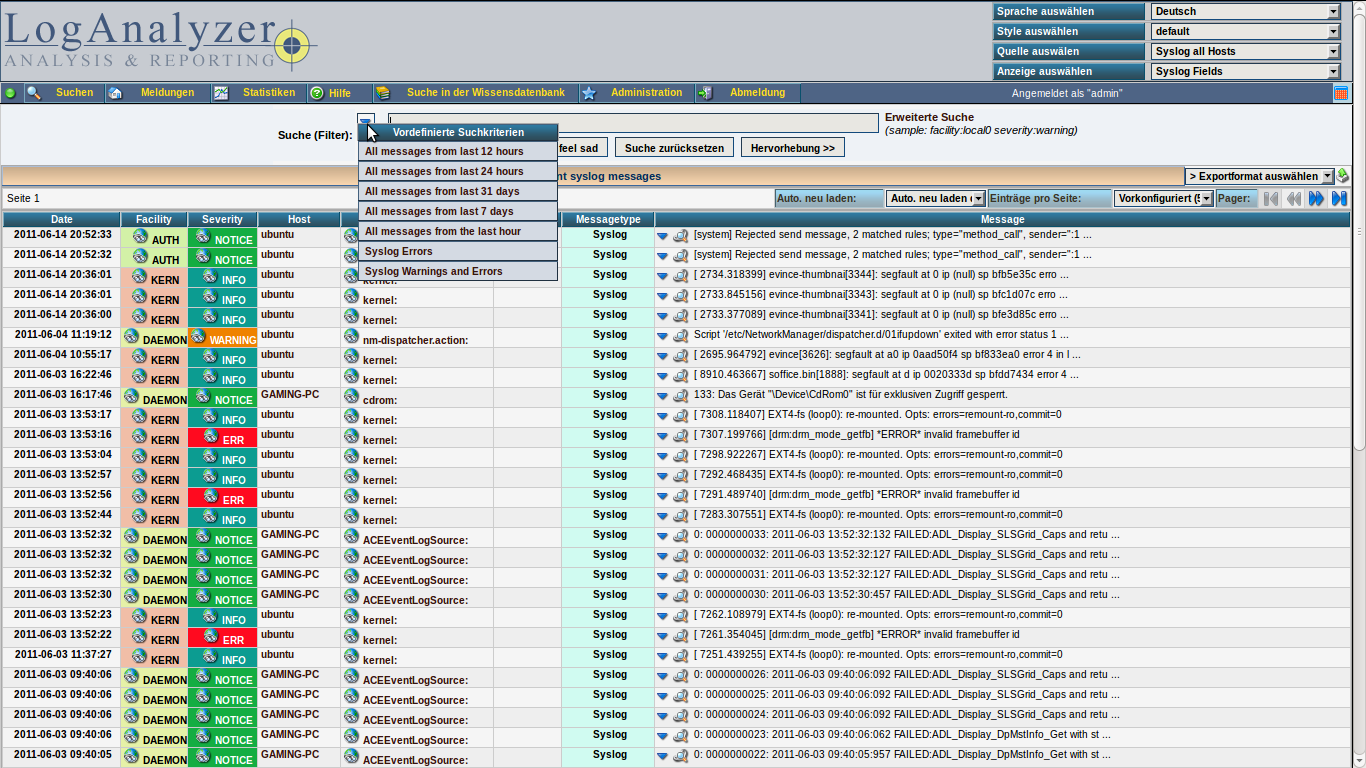
\includegraphics[width=\linewidth]{images/phplogcon_meldungen.eps}
	\end{center}
\end{frame}

\subsubsection{Statistiken}
\begin{frame}
	\frametitle{phpLogCon - Webinterface}
	\framesubtitle{Statistiken}
	\begin{center}
		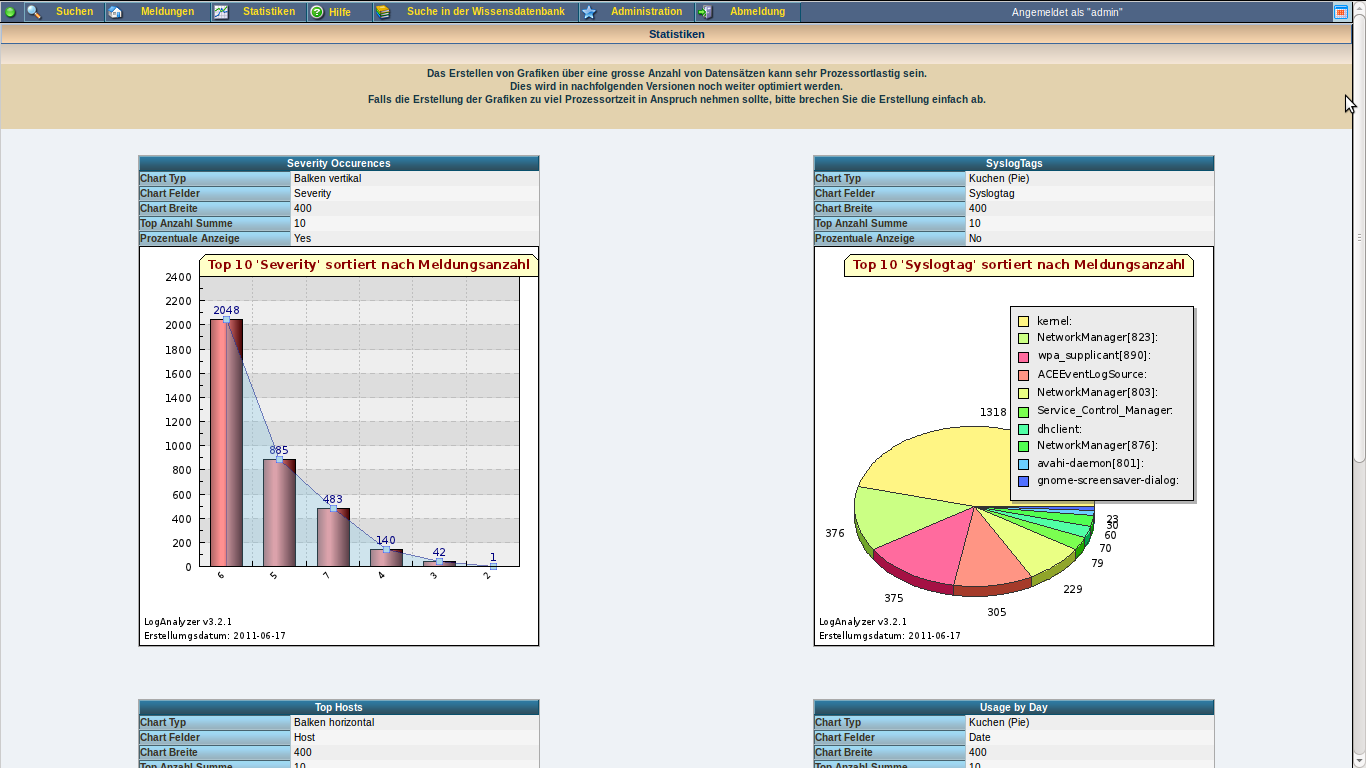
\includegraphics[width=\linewidth]{images/phplogcon_statistik.eps}
	\end{center}
\end{frame}

\subsubsection{Administration}
\begin{frame}
	\frametitle{phpLogCon - Webinterface}
	\framesubtitle{Administration}
	\begin{center}
	 	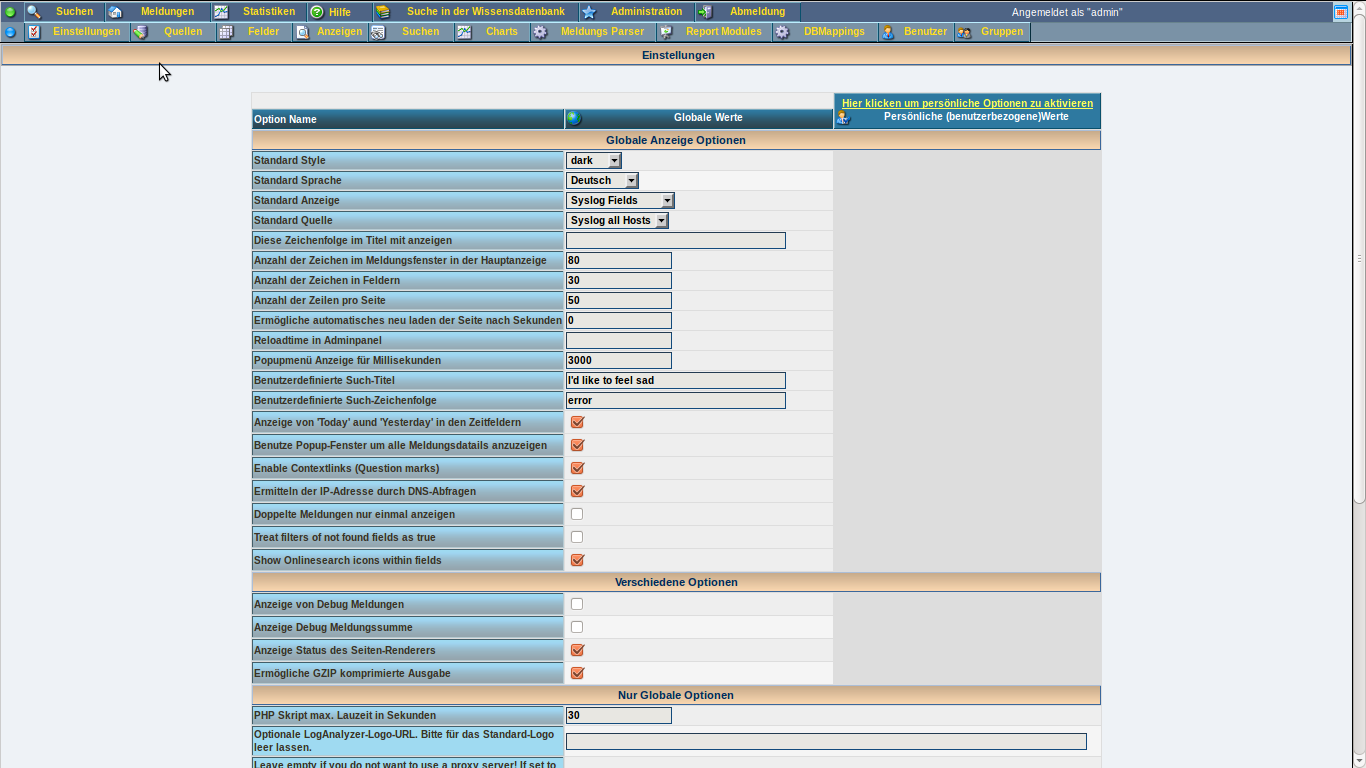
\includegraphics[width=\linewidth]{images/phplogcon_admin.eps}
	\end{center}
\end{frame}

\subsection{Alternativen}
\begin{frame}
	\frametitle{phpLogCon}
	\framesubtitle{Alternative: Logzilla}
	\begin{itemize}
		\item Vollinstallation inkl. Betriebssystem
		\item Mehr Möglichkeiten der Analyse
		\item Zusätzliche Funktionen integriert
		\item Shareware, direkter Support möglich
	\end{itemize}
\end{frame}